
In this section, we present the results of evaluation of our system. As experimental 
setup, we use RTLSDR together with signal processing algorithm implemented
in Octave. 

\subsection{Spatial variation of ambient television signals}

\begin{figure}[h]
	\centering
	\begin{minipage}{0.49\columnwidth}
	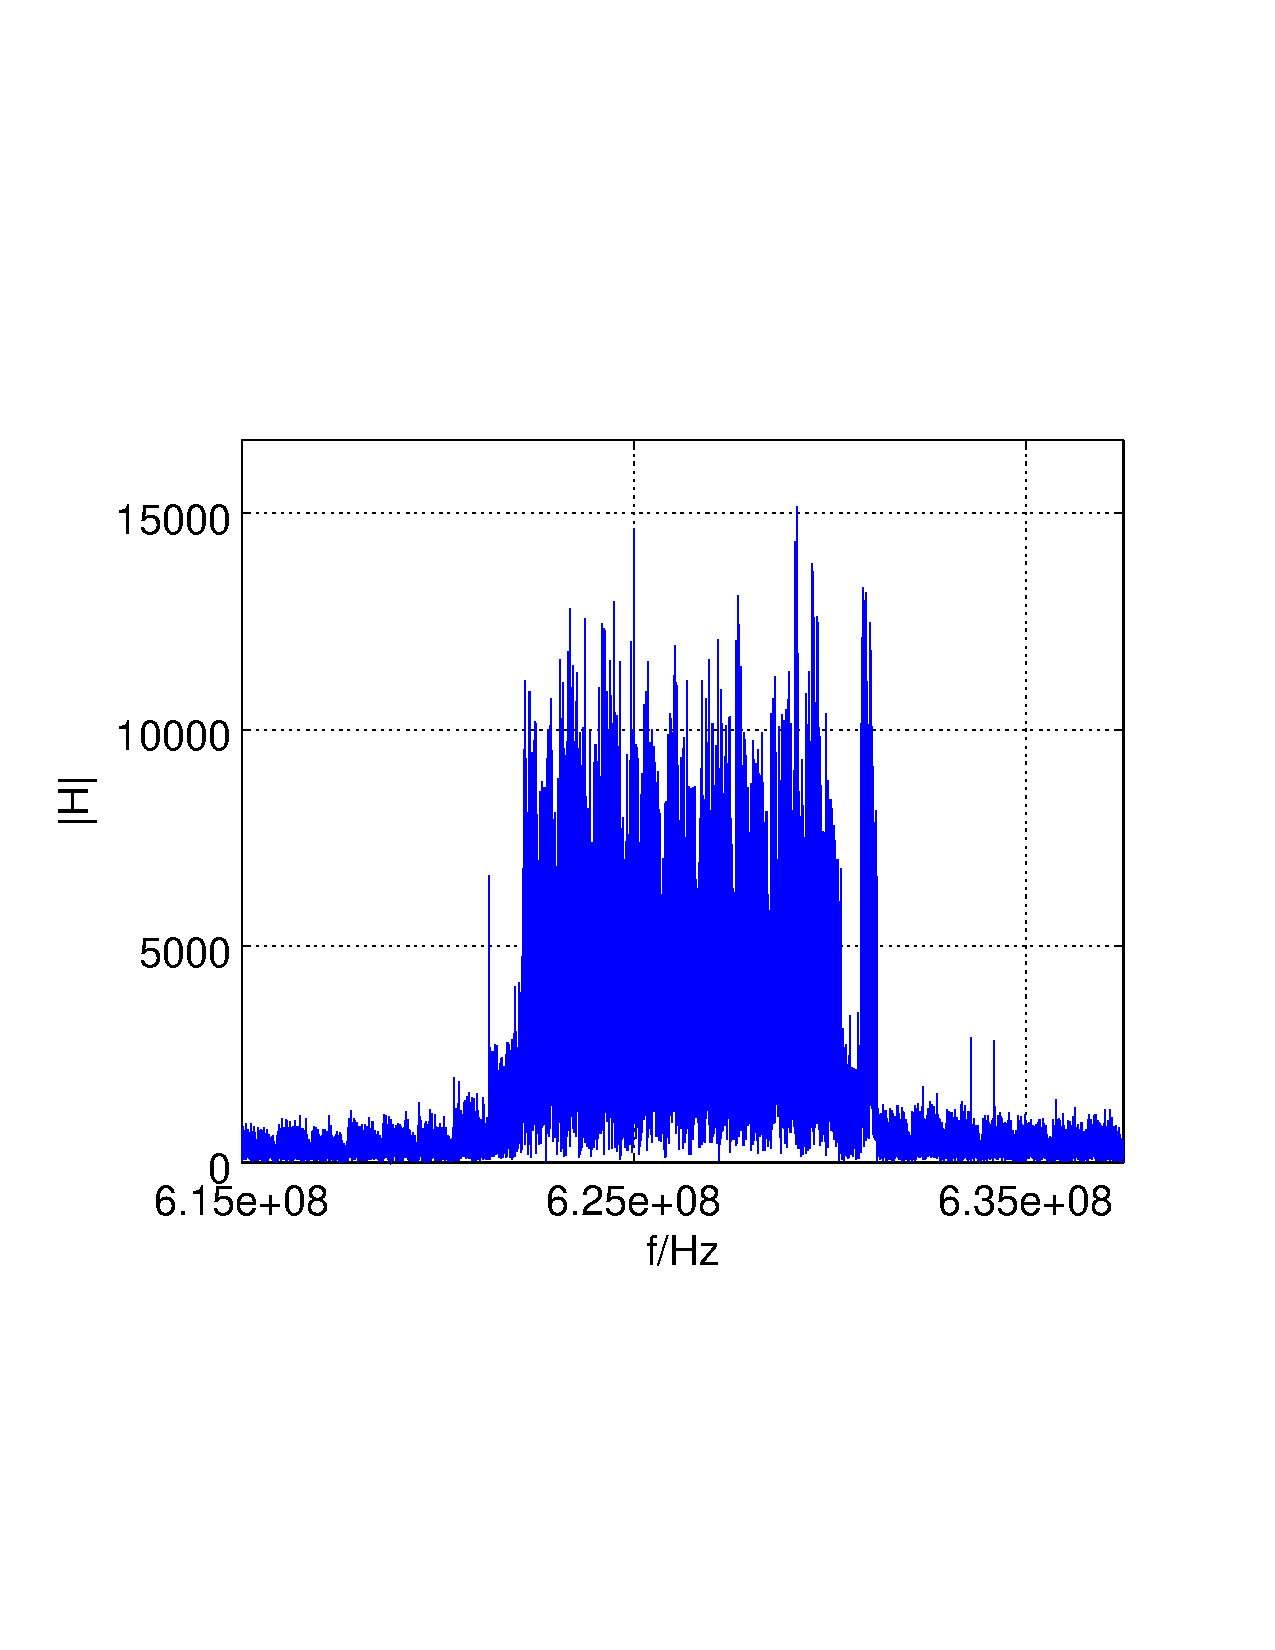
\includegraphics[width=\columnwidth]{./fig/626mhz_raw}
	\end{minipage}
	\hfill
	\begin{minipage}{0.49\columnwidth}
	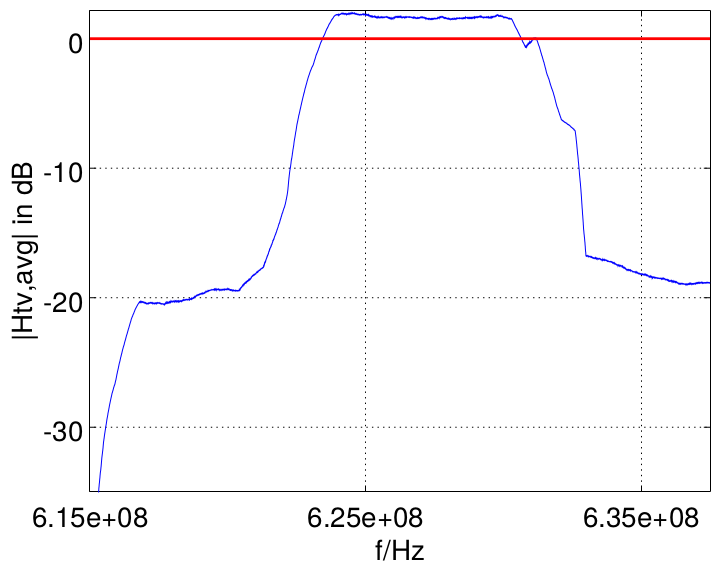
\includegraphics[width=\columnwidth]{./fig/626mhz_filtered}
	\end{minipage}
	\vspace{-6mm}
	\caption{\emph{Observed spectrum of television signal}. The left hand image shows the raw spectrum of the TV signal, with centre frequency of \SI{626}{\mega\hertz}. The right hand image shows the smoothed spectrum normalized to maximum average. The average is  shown by the horizontal red line.}
	\label{fig:tv_record} 
		\vspace{-6mm}
\end{figure}

We have used the \textit{RTL-SDR} to observe the space variations of the
signal strength. \textit{Octave} scripts have been written to aid in
this purpose. These scripts are available under \cite{s3xm3x_RTLSDRSpecAn}. The scripts perform a
frequency sweep through the desired band. The obtained samples are then
transferred from the time domain to the frequency domain using a fast
fourier transformation (FFT). 

Because the RTL-SDR has a maximum (stable) sampling rate of 2.4 MS/s, we are
limited to a maximum simultaneous acquisition band of 1.2 MHz. We keep a safety
margin to the maximum capabilities and sample the desired frequency band at 900
kHz intervals and stitch these bands together to form the overall frequency
sweep. This approach is valid only because we are not interested in real-time
data.  With this approach we are able to scan a 20 MHz band in roughly 30
seconds.

During the scanning process the gain is set to 40.2 dB. To get the
signal strength we simply take the average over a 10 MHz band around the
center frequency of the desired TV signal. This approach can be
justified by the fact, that DVB-T is specified up to 10 MHz bandwidth.
And the local TV provider advertises to be transmitting DVB-T 2.
The signal \ensuremath{|H|} is calculated as follows.  
\begin{equation}
	|H| = \Biggl| \sum_{n=0}^N FFT\biggl( \Re\{ s_{\text{band,n}}(t) \} \biggr) \Biggr|
\end{equation}     where \ensuremath{N} is the total number of intervals
accumulated over the entire frequency sweep. The FFT is only carried out over
the real values, which are received from the \textit{RTL-SDR}.
\ensuremath{s_{\text{band,n}}(t)} is the signal in the time domain of one
interval (one subband). There are as many samples taken in one band as needed
for an FFT of size 2048. To finally get \ensuremath{|H_{tv,avg}|} one has to
normalize everything and calculate the power. Before doing that, a simple
smoothing algorithm (FIR) is applied on \ensuremath{|H|}.  
\begin{equation}
	|H_{\text{tv,avg}}| = 20 \cdot log (|H|) - 20 \cdot log(|H_0|)
\end{equation}   
where \ensuremath{|H_0|} is a normalization value measured at a certain point
in space. The result of combining measured signal strength values with the
haversine function to calculate the distance to the point where the maximum
signal has been captured can be observed in Figure \ref{fig:haversine}.
\begin{figure}[h]
	\centering
	\begin{minipage}{0.49\columnwidth}
	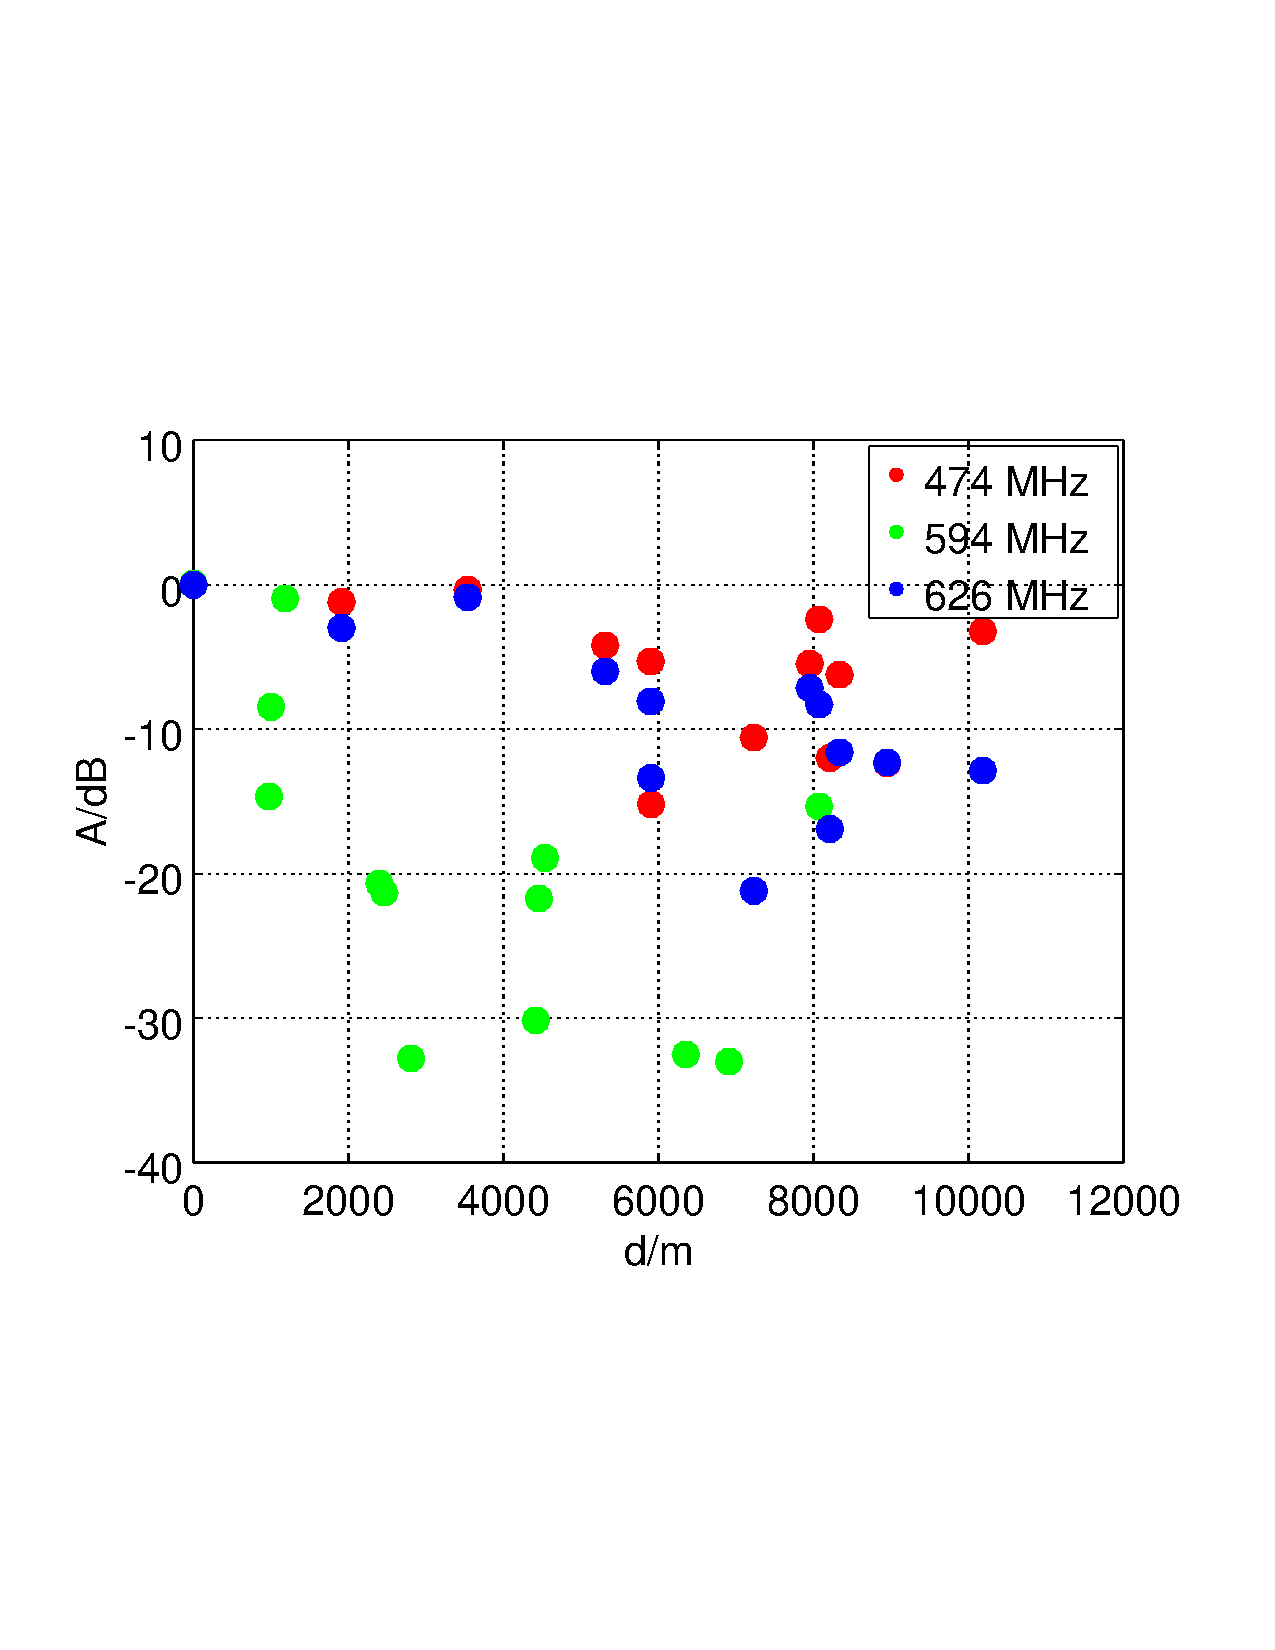
\includegraphics[width=\columnwidth]{./fig/haversine}
	\end{minipage}
	\hfill
	\begin{minipage}{0.49\columnwidth}
	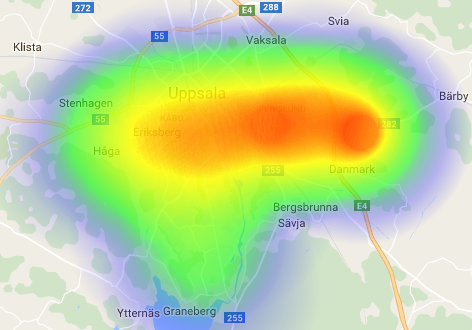
\includegraphics[width=\columnwidth]{./fig/heatmap_626mhz}
	\end{minipage}
	\vspace{-6mm}
	\caption{\emph{Spatial variation of TV signals in Uppsala city}. 
	The left image demonstrates the signal strength of TV signal fading	
	as opposed to observed signal strength near the TV tower. 
	%474 MHz and 626 MHz belong to a tower in Uppsala, Vedyxa and
%594 MHz belongs to a tower in Uppsala, Rickomberga. 
	The right image visualises the signal strength as heatmap for the signal
	present in the \SI{626}{\mega\hertz} band. Distances have been
calculated with the Haversine formula. }
 	\vspace{-6mm}

\label{fig:haversine}
\end{figure}

\balance

\subsection{Communication Performance}
We tested the communication with different data rates from 1 bit/s up to
1 kbit/s. As can be seen in Figure \ref{fig:transmission} the signal
strength from the backscatter transmitter is rather low. This leads to a
significant amount of quantization noise to appear. This situation can
be improved by increasing the analog gain of the receiver. The
transmission shown in Figure \ref{fig:transmission} was carried out with
the maximum gain (50 dB) available to our receiver. 

With a data rate of 1 bit/s, we were able to achieve a range indoors
of a couple of meters. With higher bitrates we
can only communicate over a range of a few decimeters and the 
bit error rate is still approximately 40 \%. The communication
experiment was also carried out outside, where we got similar results.  